\documentclass[aspectratio=169,11pt]{beamer}
\usepackage{graphicx}
\usepackage{booktabs}
\usepackage{tikz}
\usetikzlibrary{arrows.meta,calc,decorations.pathreplacing}

\setbeamertemplate{navigation symbols}{}
\setbeamertemplate{footline}[frame number]
\setbeamertemplate{itemize items}[circle]
\setbeamercolor{frametitle}{fg=black}
\setbeamercolor{title}{fg=black}
\setbeamercolor{structure}{fg=black!70}
\setbeamerfont{frametitle}{series=\bfseries}
\definecolor{accent}{RGB}{200,60,40}
\newcommand{\hl}[1]{\textcolor{accent}{#1}}

\title{Planets or binary stars?}
\subtitle{Finding planets with Gaia, and the impostors that look like them}
\author{SRMP 2026}
\date{}

\begin{document}

\begin{frame}
\titlepage
\end{frame}

%----------------------------------------------------------------------
\begin{frame}{Recap: the path of a star}
\centering
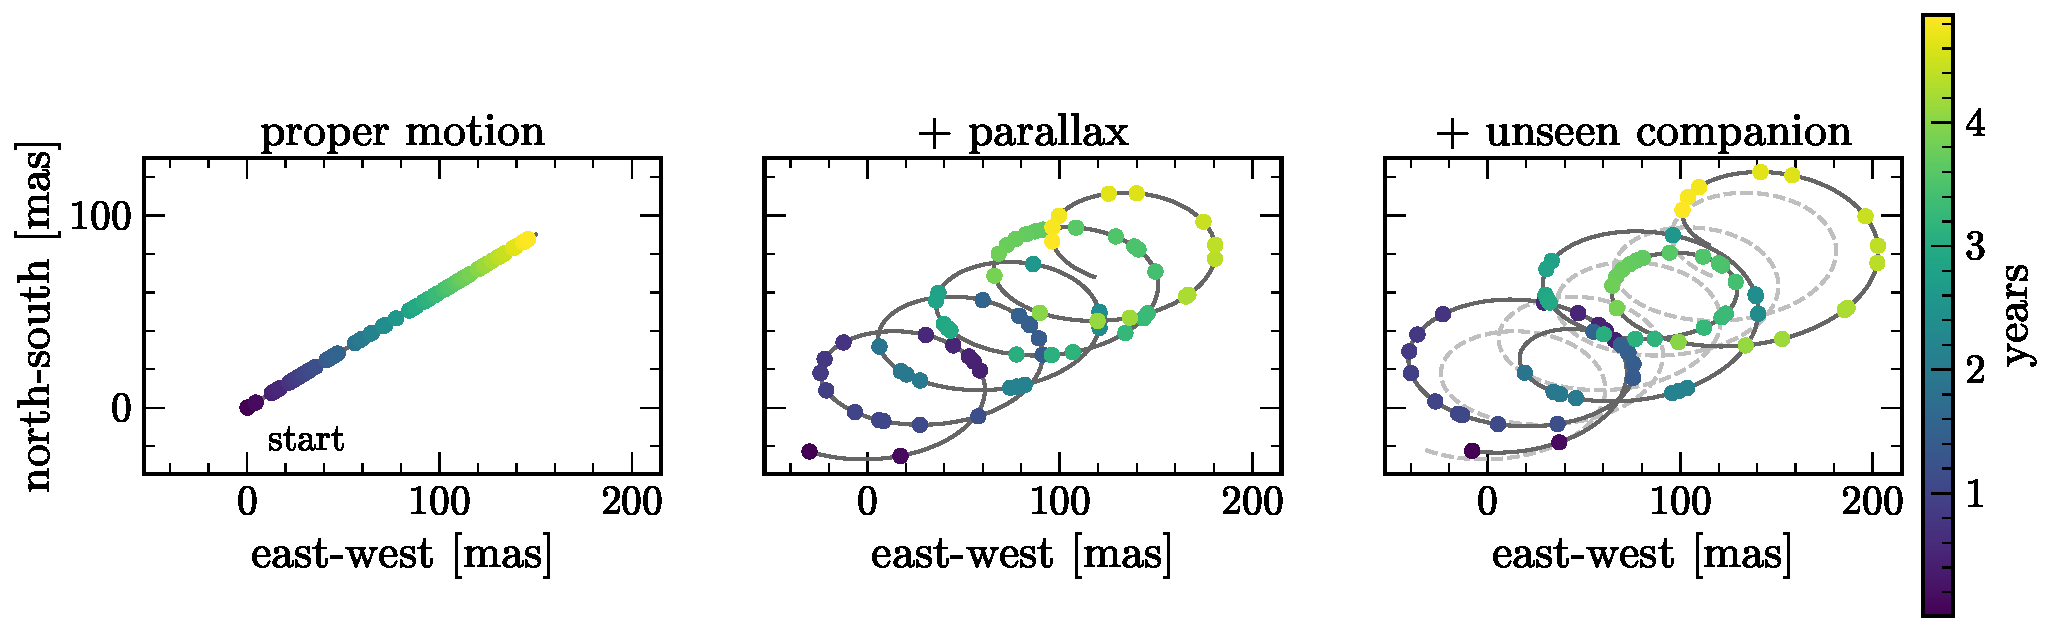
\includegraphics[width=0.95\textwidth]{figures/star_track.pdf}\\
\vspace{0.3em}
\small
Straight-line drift, plus a yearly loop from parallax. An unseen companion adds a wobble.
That wobble is how Gaia finds planets.
\end{frame}

%----------------------------------------------------------------------
\begin{frame}{Planets make their star wobble}
\begin{columns}[c]
\column{0.5\textwidth}
\centering
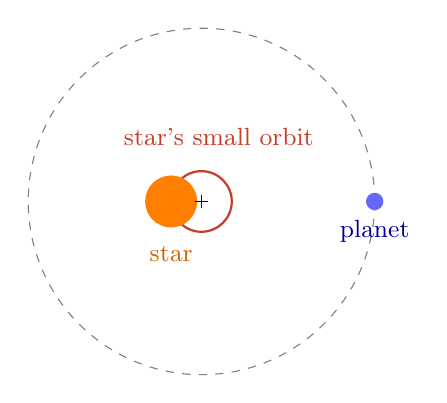
\begin{tikzpicture}[scale=1.1]
  \draw[gray,dashed] (0,0) circle (2.0);
  \draw[accent,thick] (0,0) circle (0.35);
  \fill[orange] (-0.35,0) circle (0.3);
  \fill[blue!60] (2.0,0) circle (0.1);
  \draw (0,-0.08) -- (0,0.08); \draw (-0.08,0) -- (0.08,0);
  \node[orange!80!black] at (-0.35,-0.6) {\small star};
  \node[blue!60!black] at (2.0,-0.35) {\small planet};
  \node[accent] at (0.2,0.75) {\small star's small orbit};
\end{tikzpicture}
\column{0.5\textwidth}
\begin{itemize}
\item The planet doesn't just orbit the star. Both orbit their shared balance point (center of mass).
\item So the star moves in a small circle too.
\item Bigger wobble for: heavier planets, wider orbits, lighter stars, closer stars.
\end{itemize}
\vspace{0.5em}
\begin{tabular}{lr}
\toprule
seen from 10\,pc & wobble \\
\midrule
Sun, pulled by Jupiter & 500\,$\mu$as \\
Sun, pulled by Earth & 0.3\,$\mu$as \\
\midrule
Gaia's best & $\sim$20\,$\mu$as \\
\bottomrule
\end{tabular}\\[0.3em]
\small 1\,$\mu$as = 0.001\,mas. Gaia can see Jupiters, not Earths.
\end{columns}
\end{frame}

%----------------------------------------------------------------------
\begin{frame}{Wobbles found in DR3}
\begin{columns}[c]
\column{0.5\textwidth}
\centering
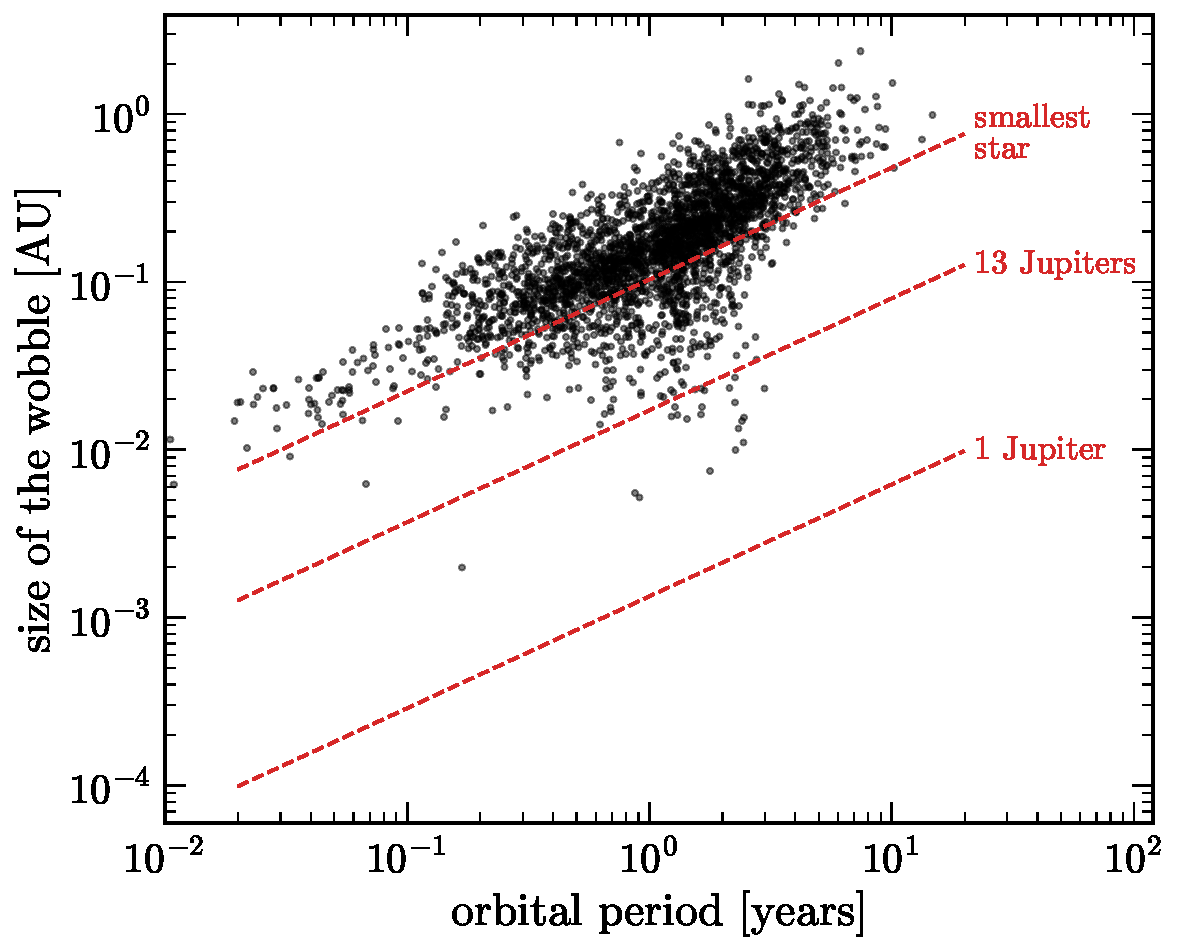
\includegraphics[width=\linewidth]{figures/dr3_orbits.pdf}
\column{0.5\textwidth}
\begin{itemize}
\item Each dot: a star within 100\,pc where Gaia found an orbit. Wobble size in AU
      (1\,AU = Earth--Sun distance).
\item Dashed lines: the wobble a dark companion would cause, for a star a bit smaller than the
      Sun. A planet would sit below the 13-Jupiter line.
\item Almost all of these are pairs of stars, not planets.
\item DR3 only published the clearest orbits. DR4 will release every measurement, so we can search all stars ourselves.
\end{itemize}
\end{columns}
\end{frame}

%----------------------------------------------------------------------
\begin{frame}{The problem: impostors}
\begin{columns}[c]
\column{0.5\textwidth}
\begin{itemize}
\item Two stars that are too close together look like one dot to Gaia.
\item Gaia sees the center of their \emph{light}. Both stars orbit the center of their \emph{mass}.
\item Heavier stars are much brighter, so the light center sits close to the heavier star.
      Unequal pair: a big wobble, an obvious binary.
\item If the two stars are \hl{almost twins}, the two centers almost coincide. The wobble is
      tiny, and looks just like a planet.
\end{itemize}
\column{0.5\textwidth}
\centering
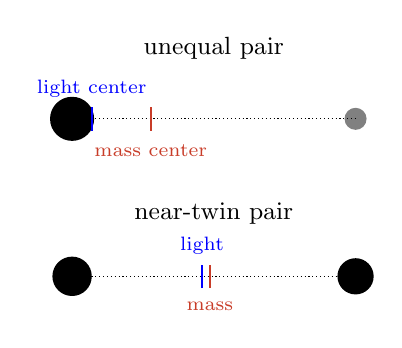
\begin{tikzpicture}[scale=1]
  \node at (1.8,2.7) {\small unequal pair};
  \fill (0,1.8) circle (0.28); \fill[gray] (3.6,1.8) circle (0.14);
  \draw[densely dotted] (0,1.8) -- (3.6,1.8);
  \draw[accent,thick] (1.0,1.65) -- (1.0,1.95); \node[accent,below] at (1.0,1.6) {\scriptsize mass center};
  \draw[blue,thick] (0.25,1.65) -- (0.25,1.95); \node[blue,above] at (0.25,1.95) {\scriptsize light center};
  \node at (1.8,0.6) {\small near-twin pair};
  \fill (0,-0.2) circle (0.25); \fill (3.6,-0.2) circle (0.23);
  \draw[densely dotted] (0,-0.2) -- (3.6,-0.2);
  \draw[accent,thick] (1.75,-0.35) -- (1.75,-0.05); \node[accent,below] at (1.75,-0.4) {\scriptsize mass};
  \draw[blue,thick] (1.65,-0.35) -- (1.65,-0.05); \node[blue,above] at (1.65,-0.05) {\scriptsize light};
\end{tikzpicture}
\end{columns}
\end{frame}

%----------------------------------------------------------------------
\begin{frame}{How common are impostors?}
\begin{columns}[c]
\column{0.45\textwidth}
\centering
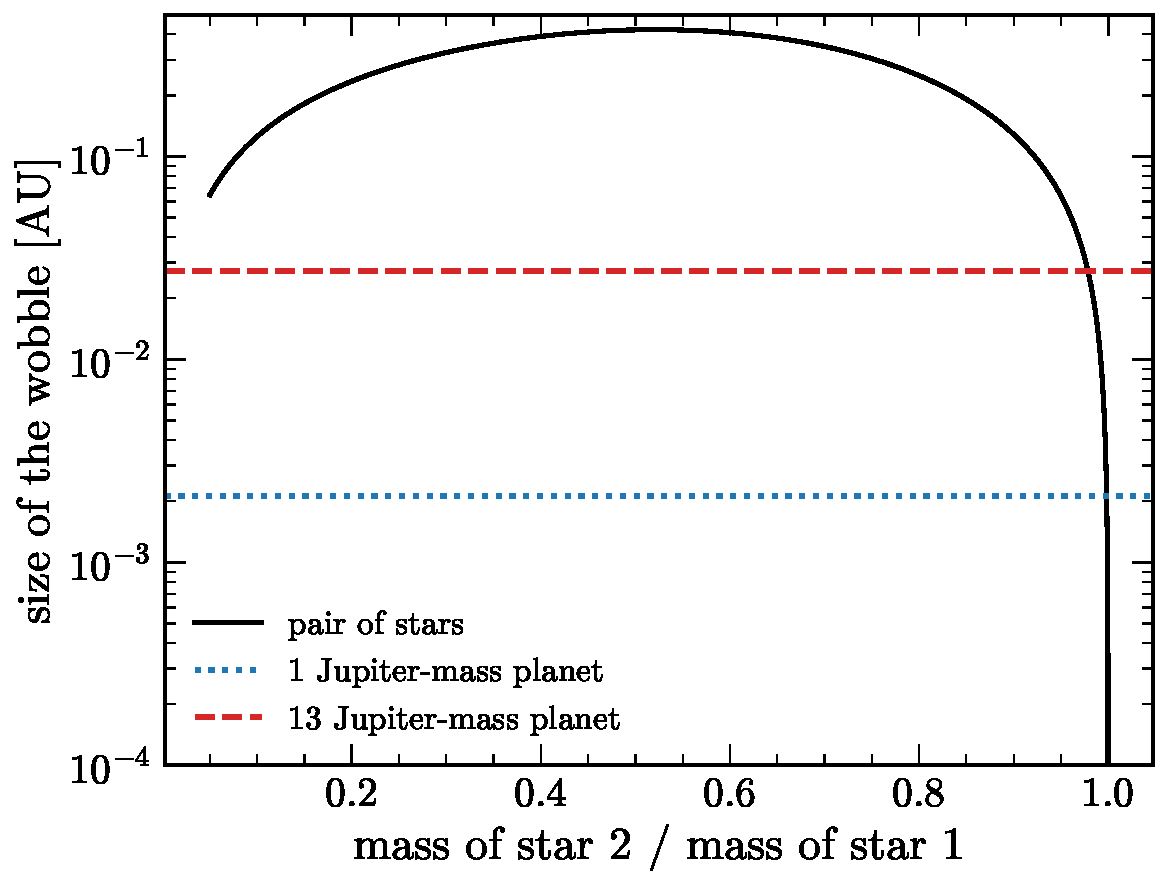
\includegraphics[width=\linewidth]{figures/impostors.pdf}
\column{0.55\textwidth}
\begin{itemize}
\item To fake a planet, the two stars must have almost the same mass: within 2\% to fake a heavy planet, within 0.2\% to fake Jupiter.
\item That sounds rare, but pairs of stars are far more common than giant planets.
\item When astronomers checked 20 DR3 wobbles that looked like planets or brown dwarfs (``failed
      stars''), 13 turned out to be twin stars.
\item DR4 is expected to find thousands of planets. Some of them will be impostors.
\end{itemize}
\end{columns}
\end{frame}

%----------------------------------------------------------------------
\begin{frame}{Our project}
\begin{center}
\large How can we tell a real planet from a pair of twin stars,\\ using only Gaia data?
\end{center}
\vspace{1em}
Some ideas:
\begin{itemize}
\item Twin stars give twice the light of one star of the same colour. So they should sit above
      the main sequence on the HR diagram. Can we use that?
\item Does the shape or size of the wobble give it away?
\item Can we simulate both kinds of systems and learn to tell them apart?
\end{itemize}
\vspace{0.5em}
Plan: learn the tools, build simulations, and be ready when DR4 comes out.
\end{frame}

%----------------------------------------------------------------------
\begin{frame}{References}
\footnotesize
\begin{itemize}
\item Perryman et al.\ 2014, \textit{Astrometric exoplanet detection with Gaia}, ApJ 797, 14
\item Gaia Collaboration, Arenou et al.\ 2023, \textit{Gaia DR3: Stellar multiplicity, a teaser
      for the hidden treasure}, A\&A 674, A34
\item Holl et al.\ 2023, \textit{Gaia DR3 astrometric orbit determination with MCMC and
      genetic algorithms}, A\&A 674, A10
\item El-Badry et al.\ 2024, \textit{A generative model for Gaia astrometric orbit catalogs},
      OJAp 7, 100
\item Stef\'ansson et al.\ 2025, \textit{Gaia-4b and 5b}, AJ 169, 107
\item Marcussen et al.\ 2026, \textit{Radial velocity follow-up of Gaia astrometric substellar
      companions: six confirmed brown dwarfs and 13 impostor binaries}, A\&A, in press
\item Lammers \& Winn 2026, \textit{On the exoplanet yield of Gaia astrometry}, AJ 171, 18
\end{itemize}
\vspace{0.5em}
Orbit plots made from Gaia DR3 data with the tutorial notebooks.
\end{frame}

\end{document}
